\documentclass[a4paper,12pt]{extarticle}
\usepackage[utf8x]{inputenc}
\usepackage[T1,T2A]{fontenc}
\usepackage[russian]{babel}
\usepackage{hyperref}
\usepackage{indentfirst}
\usepackage{listings}
\usepackage{color}
\usepackage{here}
\usepackage{array}
\usepackage{multirow}
\usepackage{graphicx}
\usepackage{algorithm}
\usepackage{algpseudocode}
\usepackage{caption}
\usepackage{pdfpages}
\usepackage{tikz,mathpazo}
\usepackage{graphicx,amssymb,amstext,amsmath,newtxmath}
\usetikzlibrary{shapes.geometric, arrows}
\renewcommand{\lstlistingname}{Программа} % заголовок листингов кода

\bibliographystyle{ugost2008ls}

\usepackage{listings}
\lstset{ %
extendedchars=\true,
keepspaces=true,
language=C,						% choose the language of the code
basicstyle=\footnotesize,		% the size of the fonts that are used for the code
numbers=left,					% where to put the line-numbers
numberstyle=\footnotesize,		% the size of the fonts that are used for the line-numbers
stepnumber=1,					% the step between two line-numbers. If it is 1 each line will be numbered
numbersep=5pt,					% how far the line-numbers are from the code
backgroundcolor=\color{white},	% choose the background color. You must add \usepackage{color}
showspaces=false				% show spaces adding particular underscores
showstringspaces=false,			% underline spaces within strings
showtabs=false,					% show tabs within strings adding particular underscores
frame=single,           		% adds a frame around the code
tabsize=2,						% sets default tabsize to 2 spaces
captionpos=t,					% sets the caption-position to top
breaklines=true,				% sets automatic line breaking
breakatwhitespace=false,		% sets if automatic breaks should only happen at whitespace
escapeinside={\%*}{*)},			% if you want to add a comment within your code
postbreak=\raisebox{0ex}[0ex][0ex]{\ensuremath{\color{red}\hookrightarrow\space}},
texcl=true,
inputpath=listings,                     % директория с листингами
}

\usepackage[left=2cm,right=2cm,
top=2cm,bottom=2cm,bindingoffset=0cm]{geometry}

%% Нумерация картинок по секциям
\usepackage{chngcntr}
\counterwithin{figure}{section}
\counterwithin{table}{section}

%%Точки нумерации заголовков
\usepackage{titlesec}
\titlelabel{\thetitle.\quad}
\usepackage[dotinlabels]{titletoc}

%% Оформления подписи рисунка
\addto\captionsrussian{\renewcommand{\figurename}{Рисунок}}
\captionsetup[figure]{labelsep = period}

%% Подпись таблицы
\DeclareCaptionFormat{hfillstart}{\hfill#1#2#3\par}
\captionsetup[table]{format=hfillstart,labelsep=newline,justification=centering,skip=-10pt,textfont=bf}

%% Путь к каталогу с рисунками
\graphicspath{{fig/}}

%% Внесение titlepage в учёт счётчика страниц
\makeatletter
\renewenvironment{titlepage} {
 \thispagestyle{empty}
}
\makeatother


\begin{document}	% начало документа

% Титульная страница
\begin{titlepage}	% начало титульной страницы

	\begin{center}		% выравнивание по центру

		\large Санкт-Петербургский политехнический университет Петра Великого\\
		\large Физико-механический институт \\
		\large Высшая школа прикладной математики и вычислительной физики\\[3cm]
		% название института, затем отступ 6см
		\large Направление подготовки\\
		\large "01.03.02. Прикладная математика и информатика"\\[3cm]
		\huge Дисциплина "Численные методы"\\[0.5cm] % название работы, затем отступ 0,5см
		\large Отчет по лабораторной работе №3\\[0.1cm]
		\large "Решение СЛАУ итерационными методами. Метод простых итераций"\\[5cm]

	\end{center}


	\begin{flushright} % выравнивание по правому краю
		\begin{minipage}{0.25\textwidth} % врезка в половину ширины текста
			\begin{flushleft} % выровнять её содержимое по левому краю

				\large\textbf{Работу выполнил:}\\
				\large Иванова А.С.\\
				\large {Группа:} 5030102/00002\\
				
				\large \textbf{Преподаватель:}\\
				\large Курц В.В.

			\end{flushleft}
		\end{minipage}
	\end{flushright}
	
	\vfill % заполнить всё доступное ниже пространство

	\begin{center}
	\large Санкт-Петербург\\
	\large \the\year % вывести дату
	\end{center} % закончить выравнивание по центру

\end{titlepage} % конец титульной страницы

\vfill % заполнить всё доступное ниже пространство


% Содержание
\renewcommand\contentsname{\centerline{Содержание}}
\tableofcontents
\newpage



\section{Формулировка задачи}

Дана функция 
\begin{math} 
	y=\sqrt{\sin{x^{2}}}
\end{math}

Требуется построить естественный кубический сплайн на некотором отрезке с использованием равномерной сетки. Исследовать сходимость интерполяционного процесса при разном количестве узлов в сетке, расположении и гладкости функции. Сравнить результаты с интерполяционным полиномом Лагранжа.

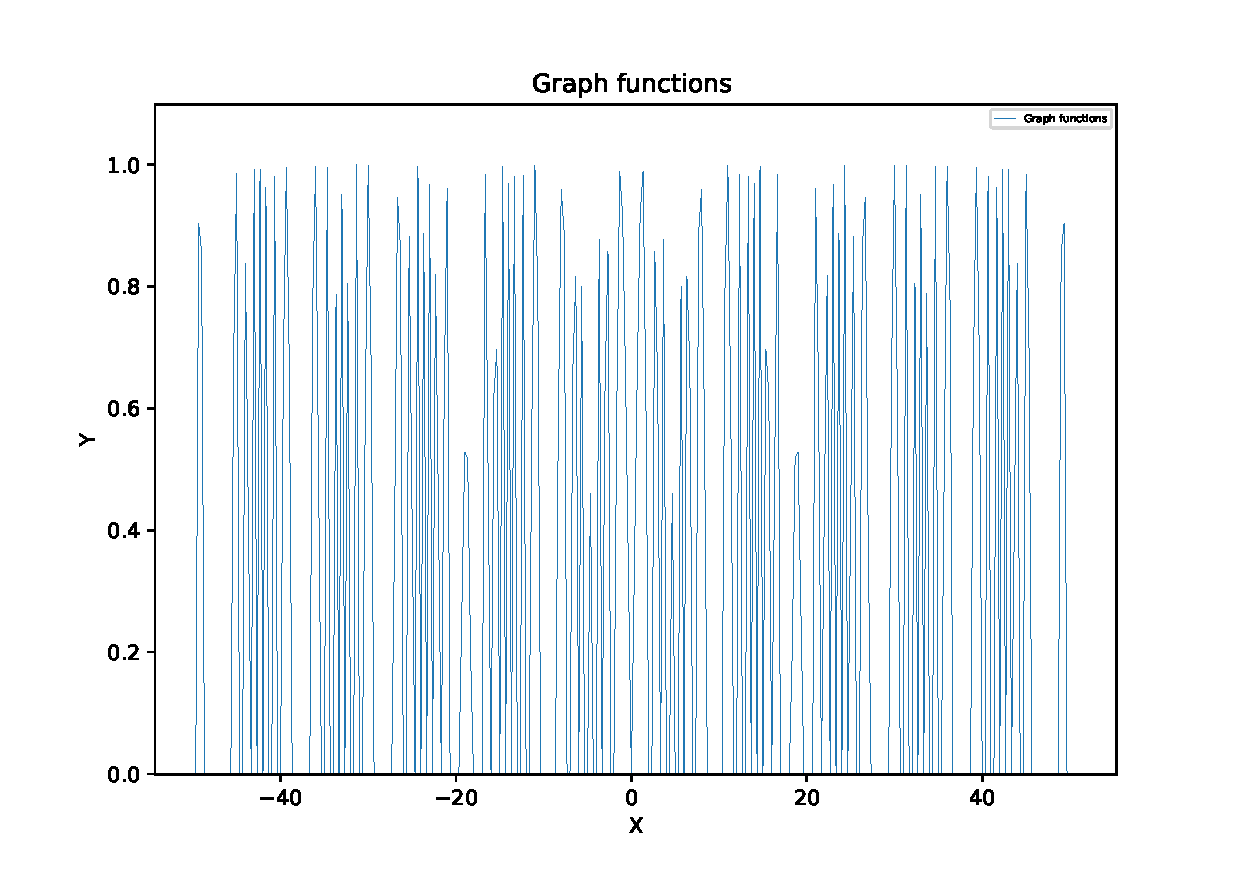
\includegraphics[scale=0.75]{graph.pdf}

\section{Алгоритм метода и условия его применимости}

\subsection{Равномерная сетка}
Дан отрезок [a,b], n - количество разбиений. Равномерная сетка 
\begin{math} 
	\{x_{i}\}_{i=0}^{n}
\end{math}
задается как: 

\begin{math} 
	x_{i}=x_{0}+\frac{(b-a)*i}{n}; i=0,...,n
\end{math}

\subsection{Алгоритм метода}

Даны некоторая сетка на отрезке [a,b]
\begin{math} 
	\{x_{i}\}_{i=0}^{n}
\end{math}
и сеточная функция
\begin{math} 
	\{y_{i}\}_{i=0}^{n}
\end{math}. 

Кубическим сплайном дефекта 1 (разность между степенью и гладкостью сплайна) называется функция 
\begin{math} 
	S(x)
\end{math}, которая на каждом отрезке является многочленом степени не выше третьей, имеет непрерывные первую и вторую производные на всём отрезке [a,b], в точках \begin{math} 
x_{i}
\end{math} выполняется равенство 
\begin{math} 
	S(x_{i})=f(x_{i})
\end{math}

Естественный сплайн имеет граничные условия вида: 

\begin{math} 
	S^{''}(a)=S^{''}(b)=0
\end{math}

Построение сплайна осуществляется следующим образом: 

На каждом отрезке 
\begin{math} 
	[x_{i-1};x_{i}], i=1,...,n
\end{math}
функция S(x) есть полином третьей степени 
\begin{math} 
	S_{i}(x)
\end{math}, коэффициенты которого надо определить. Заишем для удобства \begin{math} 
S_{i}(x)
\end{math} в виде:

\begin{math} 
	S_{i}(x)=a_{i}+b_{i}(x-x_{i})+c_{i}(x-x_{i})^{2}+d_{i}(x-x_{i})^{3}
\end{math} 

тогда

\begin{math} 
	S_{i}(x_{i})=a_{i}, S_{i}^{'}(x_{i})=b_{i},S_{i}^{''}(x_{i})=2c_{i}, S_{i}^{'''}(x_{i})=6d_{i}, i=1,...,n
\end{math}

Обозначим 
\begin{math} 
	\\
	g(x) := S_{3}^{1}(x) \\
	g_{i}(x) := S_{3}^{1}(x) |_{[x_{i-1};x_{i}]}
\end{math} 

Условия непрерывности всех производных до второго порядка включительно записываются в виде

\begin{math} 
	g_{i}(x_{i-1})=g_{i-1}(x_{i-1})
\end{math} 

\begin{math} 
	g_{i}^{'}(x_{i-1})=g_{i-1}^{'}(x_{i-1})
\end{math} 

\begin{math} 
	g_{i}^{''}(x_{i-1})=g_{i-1}^{''}(x_{i-1})
\end{math} 

где i меняется от 1 до n, а условия интерполяции в виде

\begin{math} 
	g_{i}(x_{i})=f(x_{i})
\end{math}

Обозначим 

\begin{math} 
    h_{i}=x_{i}-x_{i-1}, i=1,...,n \\
    M_{i}=g^{''}(x_{i})
\end{math}

\begin{math} 
	\\
	g_{i}^{''}(x_{i})=M_{i} \\
	g_{i-1}^{''}(x_{i-1}) = M_{i-1} \\
	g_{i}^{''}(x)=M_{i-1} \frac{x_{i}-x}{h_{i}}+M_{i}\frac{x-x_{i-1}}{h_{i}}, x\in[x_{i-1};x_{i}]
\end{math}

Если проинтегрировать дважды данное уравнение: 

\begin{math} 
	\\
	g_{i}(x)=M_{i-1}\frac{(x_{i}-x)^{3}}{6h_{i}}+M_{i}*\frac{(x-x_{i-1})^{3}}{6h_{i}}+C_{i}(x-x_{i-1})+\tilde C_{i} \\
	g_{i}(x_{i-1})=y_{i-1}=M_{i-1}\frac{h_{i}^{2}}{6}+\tilde C_{i} \\
	g_{i}(x_{i})=y_{i}=M_{i}\frac{h_{i}^{2}}{6}+ C_{i}h_{i}+ \tilde C_{i}\\
	\tilde C_{i} = y_{i-1}-M_{i-1}\frac{h_{i}^{2}}{6} \\
	C_{i}=\frac{y_{i}-y_{i-1}}{h_{i}}-\frac{h_{i}}{6}(M_{i}-M_{i-1}) \\
	M_{i}\frac{h_{i}}{2}+\frac{y_{i}-y_{i-1}}{h_{i}}-\frac{h_{i}}{6}(M_{i}-M_{i-1})=-M_{i}\frac{h_{i+1}}{2}+\frac{y_{i+1}-y_{i}}{h_{i+1}}-\frac{h_{i}}{6}(M_{i+1}-M_{i})
\end{math}

Получаем следующую систему уравнений: 

 \begin{math}
 	\\
 		\frac{h_{i}}{h_{i}+h_{i+1}}M_{i-1}+2M_{i}+\frac{h_{i+1}}{h_{i}+h_{i+1}}M_{i+1}=\frac{6}{h_{i}+h_{i+1}}(\frac{y_{i+1}-y_{i}}{h_{i+1}}-\frac{y_{i}-y_{i-1}}{h_{i}}), i=0,1,...,n-1
 \end{math}
,где
 \begin{math} 
	\\
	M_{0}=0 \\
	M_{n}=0\\
\end{math}
Данная система является трехдиагональной, решается методом прогонки для трехдиагональных матриц
 
Т.к 

\begin{math} 
	S_{i}(x_{i})=a_{i}, S_{i}^{'}(x_{i})=b_{i},S_{i}^{''}(x_{i})=2c_{i}, S_{i}^{'''}(x_{i})=6d_{i}, i=1,...,n
\end{math}

Получаем: 

\begin{math} 
	2c_{i}=M_{i}
\end{math}

На основе полученных результатов получаем формулы для вычисления коэффициентов естественного кубического сплайна:

\begin{math} 
	a_{i}=f(x_{i})
\end{math}

\begin{math} 
	d_{i}=\frac{c_{i}-c_{i-1}}{3h_{i}}
\end{math}

\begin{math} 
	b_{i}=\frac{y_{i}-y_{i-1}}{h_{i}}-\frac{2*c_{i}+c_{i-1}}{3}*h_{i}
\end{math}

где 

\begin{math} 
	c_{n}=S^{''}(x_{n})=0
\end{math}

\begin{math} 
	S^{''}(x_{0})=0
\end{math}

Вычисления с можно проводить с помощью метода прогонки для трехдиагональной матрицы


\subsection{Условия применимости метода}

Все узлы сетки попарно различны.

\section{Предварительный анализ задачи}

При выборе отрезка ненулевой длины для интерполирования получившаяся равномерная сетка может считаться упорядоченной, а значит все узлы сетки попарно различны. Значит существует интерполяционный кубический слпайн, и он единственный. 


\section{Проверка условий применимости метода}

При выборе отрезка ненулевой длины для интерполирования получившаяся равномерная сетка может считаться упорядоченной, а значит все узлы сетки попарно различны. Значит существует интерполяционный кубический слпайн, и он единственный. 



\section{Тестовый пример с детальными расчетами для задачи малой размерности}

Функция \begin{math} 
	y=\sqrt{\sin{x^{2}}}
\end{math}

Сетка : 
\begin{math} 
	\{-\sqrt{\frac{\pi}{2}};0;\sqrt{\frac{\pi}{2}}\}
\end{math}

Сеточная функция: 
\begin{math} 
	\{1;0;1\}
\end{math}

Общий вид кубического сплайна: 

\begin{math} 
	S_{i}(x)=a_{i}+b_{i}(x-x_{i})+c_{i}(x-x_{i})^{2}+d_{i}(x-x_{i})^{3}
\end{math} 

Вычисление коэффициентов: 


\begin{math} 
	\\
	a_{1}=0;a_{2}=1; c_{2}=0
\end{math}

\begin{math} 
	\\
	h_{1}=x_{1}-x_{0}=\sqrt{\frac{\pi}{2}}; \\ h_{2}=x_{2}-x_{1}=\sqrt{\frac{\pi}{2}}
\end{math}

Необходимо решить следующую систему уравнений:

\begin{math} 
	h_{i}=x_{i}-x_{i-1}, i=1,...,2 \\
	M_{i}=g^{''}(x_{i})
\end{math}

 \begin{math} 
	\\
	M_{0}=0 \\
	M_{2}=0\\
\end{math}

\begin{math}
		\frac{h_{1}}{h_{1}+h_{2}}M_{0}+2M_{1}+\frac{h_{2}}{h_{1}+h_{2}}M_{2}=\frac{6}{h_{1}+h_{2}}(\frac{y_{2}-y_{1}}{h_{2}}-\frac{y_{1}-y_{0}}{h_{1}})
\end{math}

В данном случае получается уравнение, однозначно разрешимое относительно \begin{math} 
	M_{1}
\end{math}
, поскольку две другие переменные равны 0, исходя из условия естественного кубического сплайна

Решение данного уравнения и нахождение коэффициентов сплайна: 

\begin{math} 
	\\
	\alpha_{0}=\beta_{0}=0
\end{math}

\begin{math} 
	\\
	M_{1}=\frac{3}{h_{1}+h_{2}}(\frac{y_{2}-y_{1}}{h_{2}}+\frac{y_{1}-y_{0}}{h_{1}})=\frac{3}{\pi} \\ 
	d_{1}=\frac{c_{1}-c_{0}}{3*h_{1}}=\frac{\sqrt{2}}{\pi\sqrt{\pi}} \\
	b_{1}=\frac{y_{1}-y_{0}}{h_{1}}-\frac{2*c_{1}+c_{0}}{3}*h_{1}=0 \\
	c_{2}=0 \\
	d_{2}=\frac{c_{2}-c_{1}}{3*h_{2}}=-\frac{\sqrt{2}}{\pi\sqrt{\pi}} \\
	a_{2}=1 \\
	b_{2}=\frac{y_{2}-y_{1}}{h_{2}}-\frac{2*c_{2}+c_{1}}{3}*h_{2}= \frac{1}{\sqrt{2\pi}} \\
\end{math}

Итого: 

\begin{math} 
	\\
	S_{1}(x)=\frac{3}{\pi}x^{2}+\frac{\sqrt{2}}{\pi\sqrt{\pi}}x^{3} \\
	S_{2}(x)=1+\frac{1}{\sqrt{2\pi}}(x-\sqrt{\frac{\pi}{2}})-\frac{6\sqrt{2}}{\pi\sqrt{\pi}}(x-\sqrt{\frac{\pi}{2}})^{3}
\end{math}

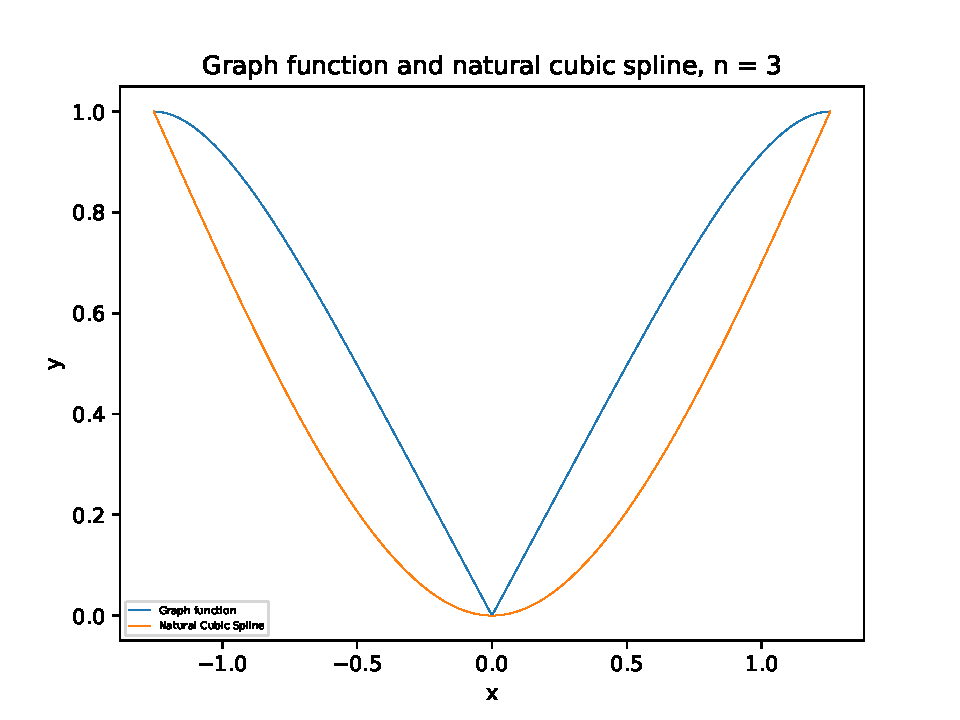
\includegraphics[scale=0.75]{13.pdf}


\section{Перечень контрольных тестов для иллюстрации метода}

Дана функция 
\begin{math} 
	y=\sqrt{\sin{x^{2}}}
\end{math}

На разных отрезках строился естественный кубический сплайн. Число узлов менялось в цикле от 3 до 100. Исследуется сходимость интерполяционного процесса (максимальное отклонение сплайна от функции от n) на разных участках при разных разбиениях и гладкости функции. Результаты сравнивались с результатами интерполяции полиномами Лагранжа на аналогичных участках с равномерной и чебышевской сеткой. 

Данная функция имеет в основном периодическую область определения, разрывов производной на области определения нет, производная не существует на тех участках, где не существует действительных знаечний исходной функции. 

Существует единственный разрыв производной в области опеределения - это точка [0,0]

Рассматривались участки, принадлежащие области определния функции: 

1) [-1.5;1.5], на данном участке присутсвует разрыв производной. 

2) \begin{math} 
	[\sqrt{300*\pi}; \sqrt{301*\pi}]
\end{math}

2) \begin{math} 
	[\sqrt{700*\pi}; \sqrt{701*\pi}]
\end{math}

\section{Модульная структура программы}


def my\_func(x):

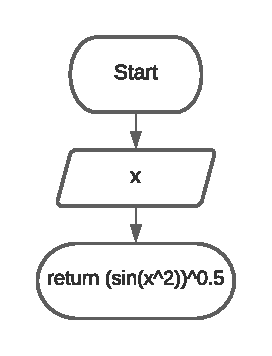
\includegraphics[scale=0.7]{block1.pdf}

def func\_values(func, xlist):

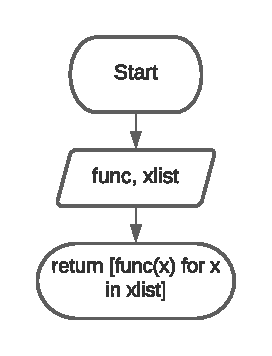
\includegraphics[scale=0.75]{block2.pdf}

def spline(x, y, n):

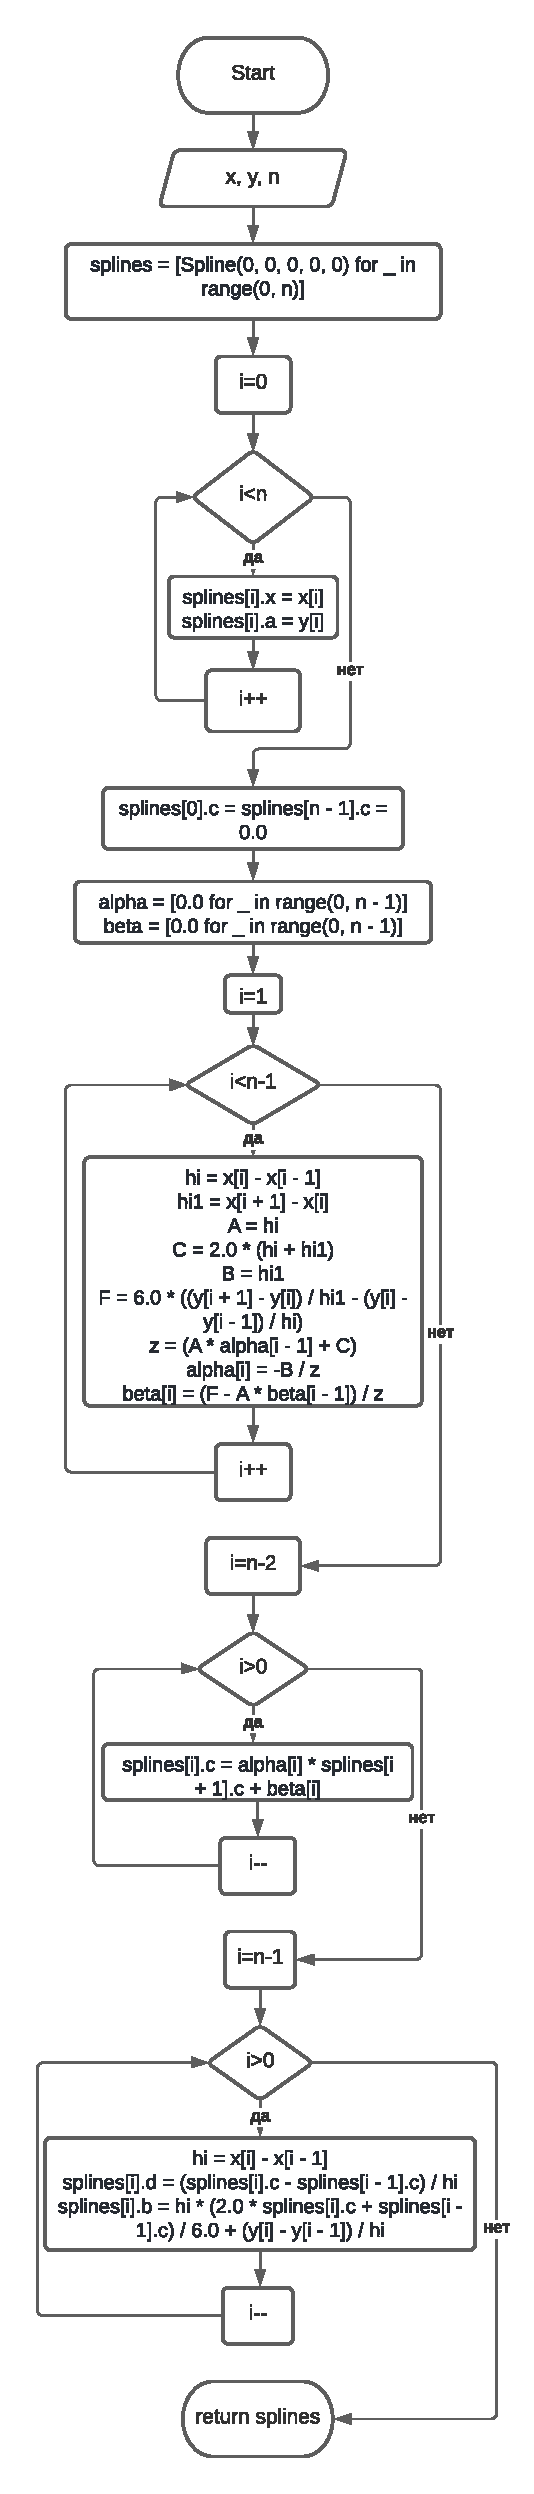
\includegraphics[scale=0.55]{block3.pdf}

def interpolate(splines, x):

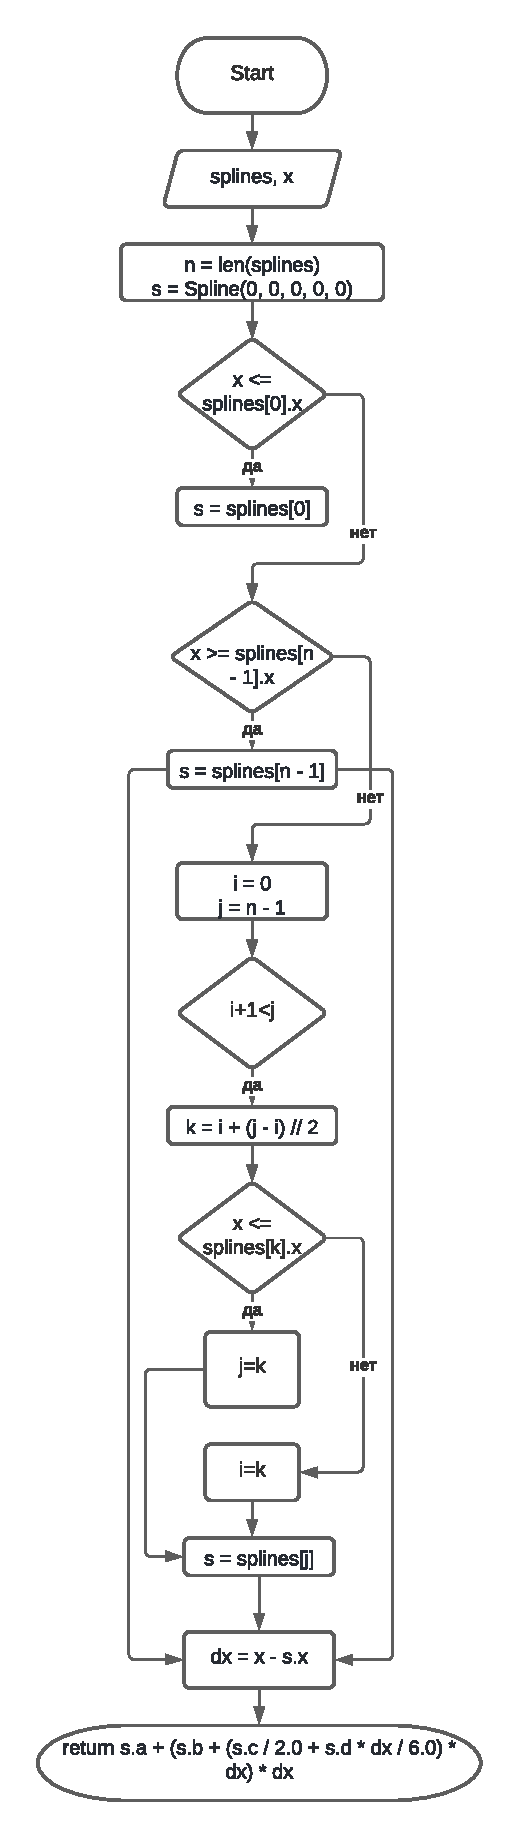
\includegraphics[scale=0.75]{block4.pdf}

\section{Численный анализ решения задачи}

\subsection{\begin{math}[-1.5;1.5]
\end{math}}

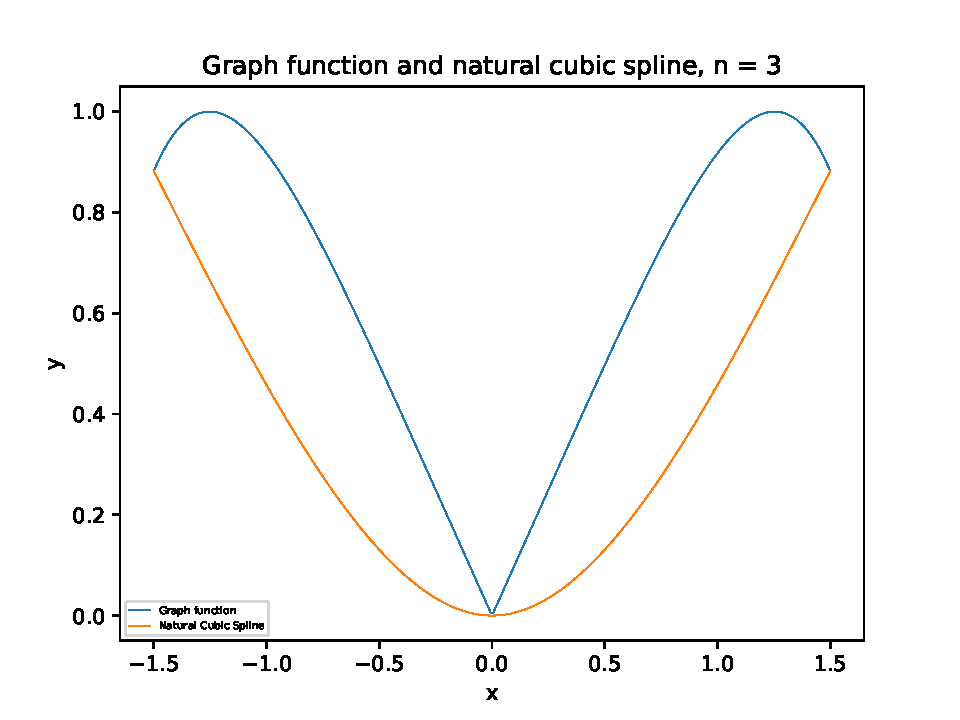
\includegraphics[scale=0.75]{1.pdf}

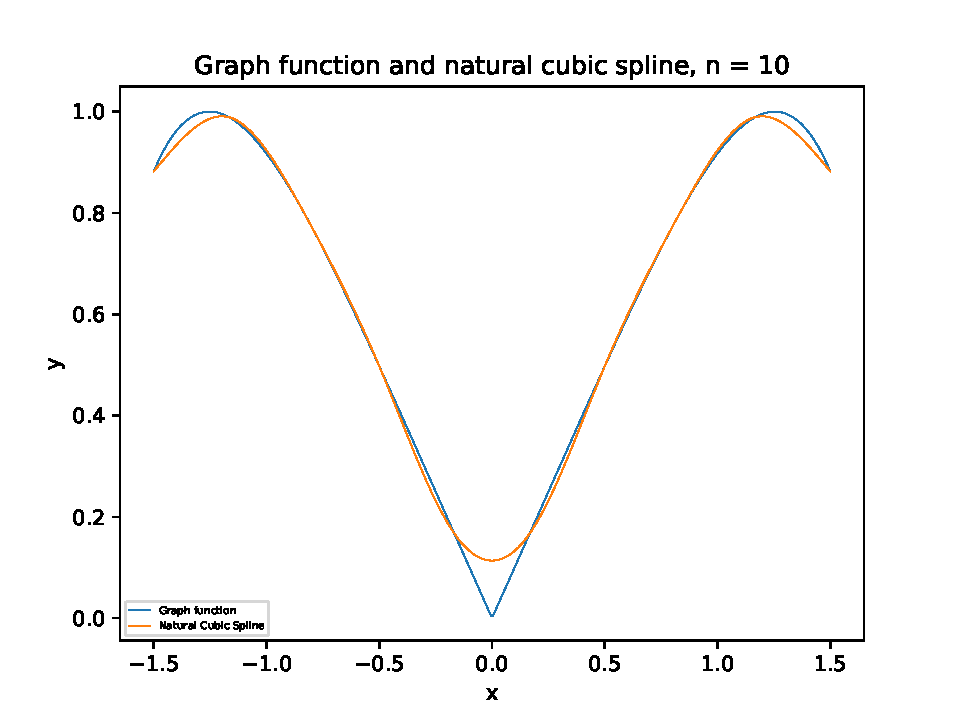
\includegraphics[scale=0.75]{2.pdf}

На данных графиках изображены кубические сплайны при двух различных количествах узлов. Из графиков видно, что при увеличении числа узлов погрешность уменьшается. Погрешность остается большой в области разрыва производной.

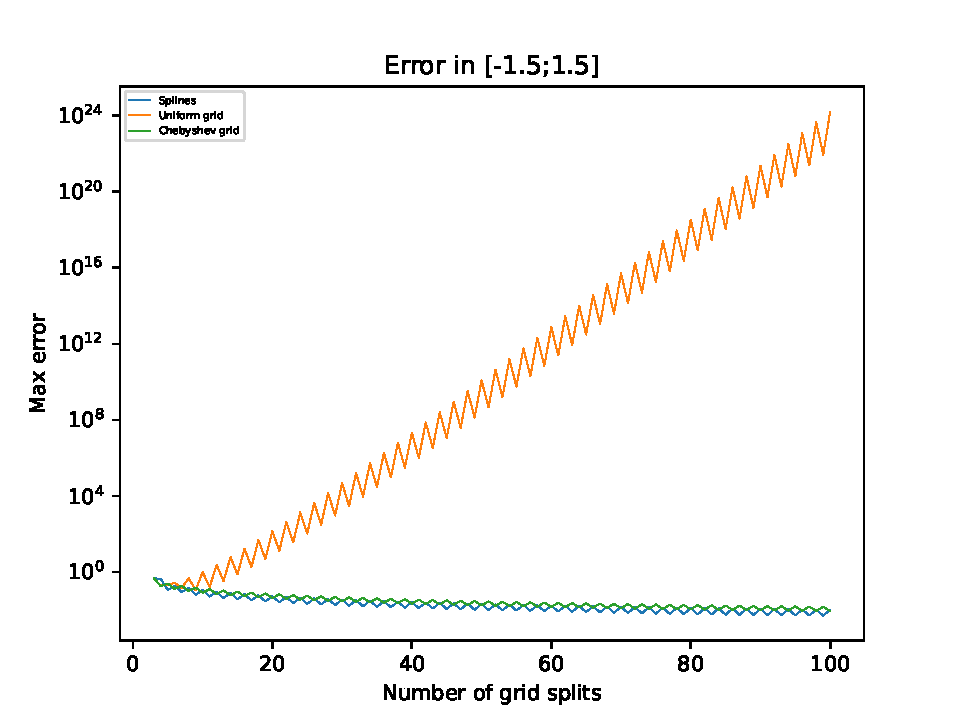
\includegraphics[scale=0.75]{10.pdf}

На данном графике изображена сходимость интерполяционного процесса для полинома Лагранжа с равномерной и чебышевской сеткой и естественного кубического сплайна. Сплайн и полином с сеткой Чебышева дают примерно одинаковый результат.

\subsection{ \begin{math} 
		[\sqrt{300*\pi}; \sqrt{301*\pi}]
\end{math}}

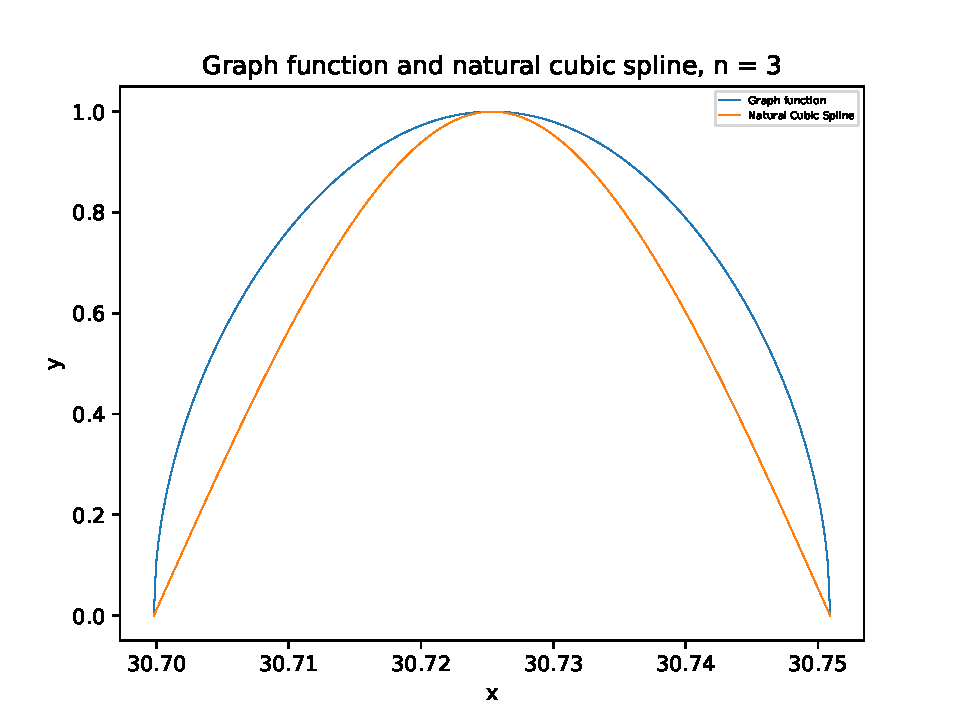
\includegraphics[scale=0.75]{3.pdf}

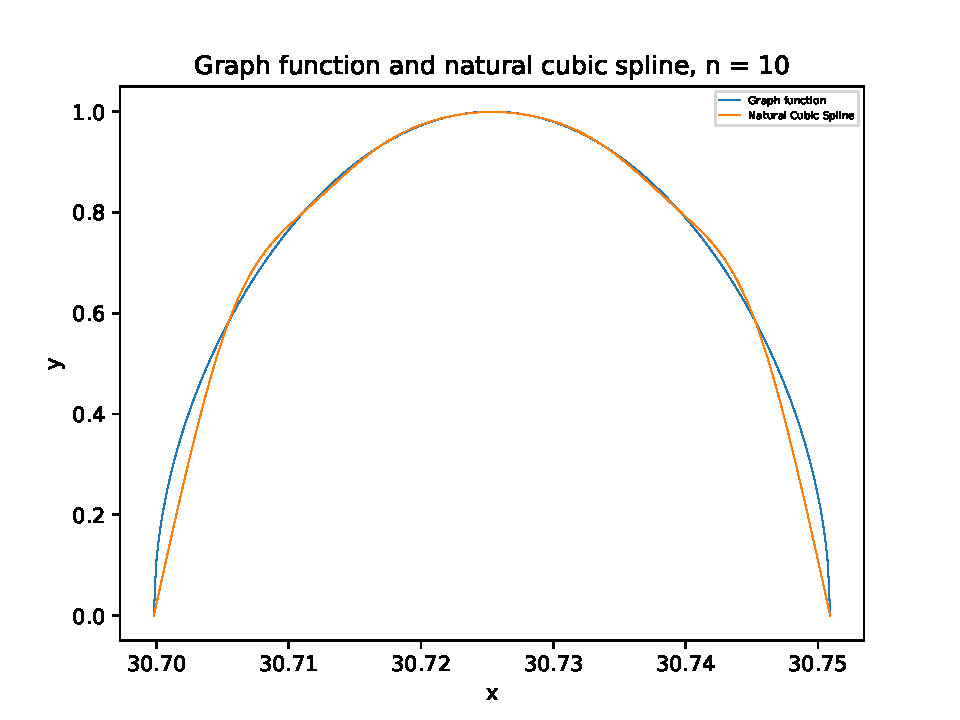
\includegraphics[scale=0.75]{4.pdf}

На данных графиках изображены кубические сплайны при двух различных количествах узлов. Из графиков видно, что при увеличении числа узлов погрешность уменьшается.

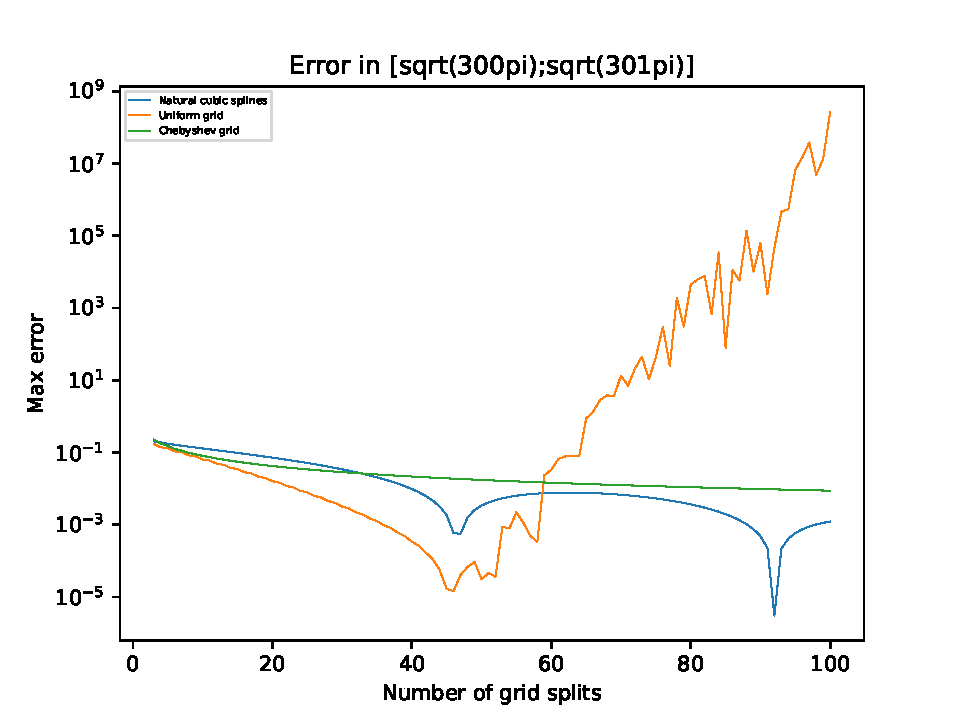
\includegraphics[scale=0.75]{11.pdf}

На данном графике изображена сходимость интерполяционного процесса для полинома Лагранжа с равномерной и чебышевской сеткой и естественного кубического сплайна. Сплайны дают результат чуть лучше, чем полиномы с сеткой Чебышева. Погрешность для кубического сплайна уменьшается быстрее на участке функций без разрыва производной. 

\subsection{ \begin{math} 
		[\sqrt{700*\pi}; \sqrt{701*\pi}]
\end{math}}

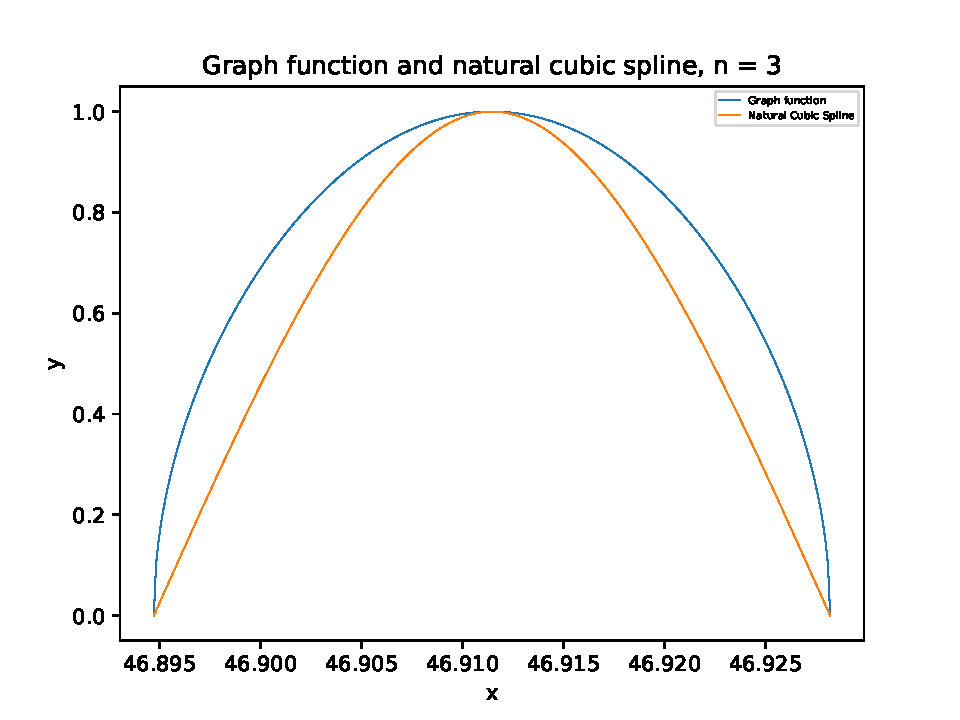
\includegraphics[scale=0.75]{5.pdf}

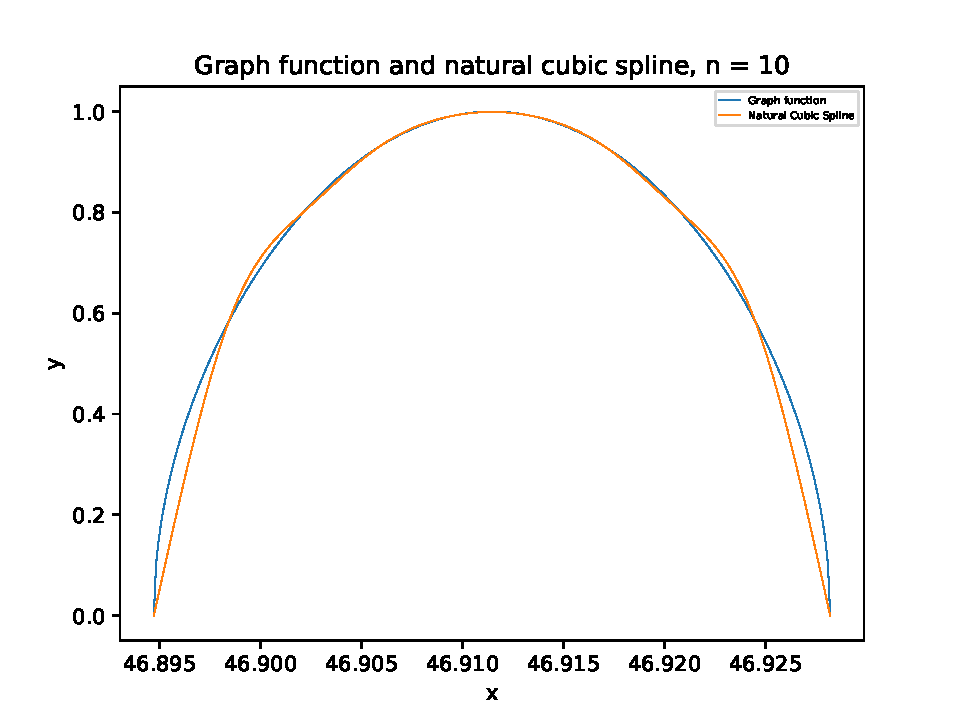
\includegraphics[scale=0.75]{6.pdf}

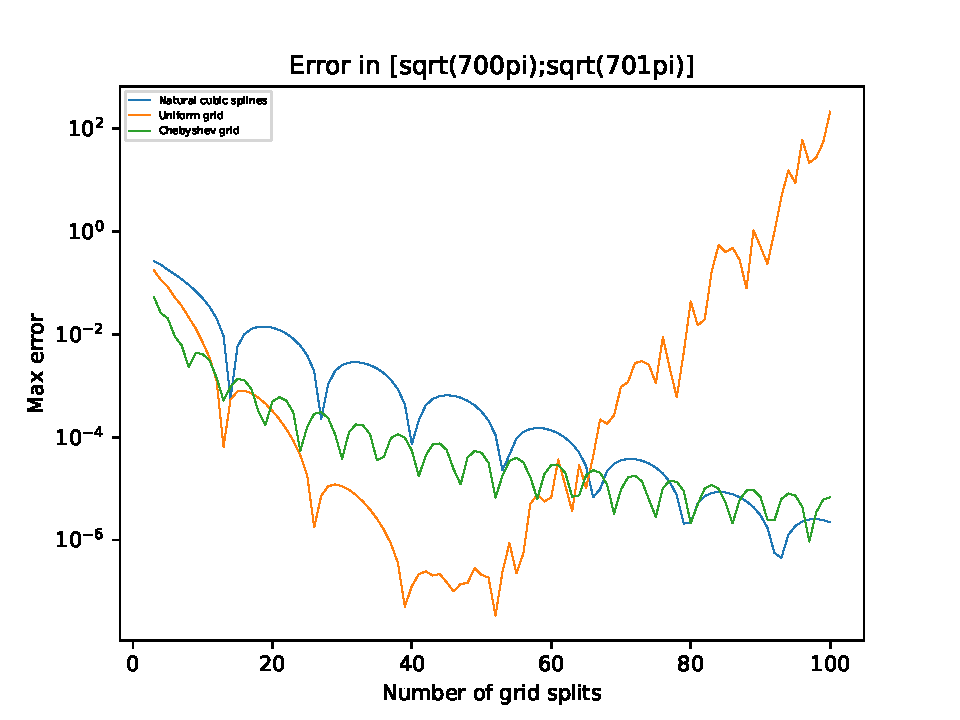
\includegraphics[scale=0.75]{12.pdf}

Да данных графиках сохраняются все ранее полученные результаты для второго интервала, за исключением того, что кубический сплайн показывает результаты чуть хуже, чем полином Лагранжа с сеткой Чебышёва.

\section{Краткие выводы}

На основе полученных результатов можно сделать вывод, что при увеличении числа узлов для естественного кубического сплайна с равномерной сеткой погрешность постепенно уменьшается. Результаты интерполяции кубическим сплайном с равномерной сеткой похожи на результаты интерполяции полиномом Лагранжа с сеткой Чебышева. 

Гладкость функции также влияет на сходимость интерполяционного процесса. Максимальное отклонение достигает наибольших значений близко к точке разрыва производной.


\end{document}
